\documentclass{article}
\usepackage[utf8]{inputenc}
\usepackage{graphicx}
\usepackage[super,negative]{nth}
\usepackage{longtable}
\usepackage{multirow}
\usepackage{fancyhdr}
\usepackage{float}
\usepackage{subfig}
\usepackage{color, soulutf8}
\usepackage{graphicx}
\usepackage{grffile}

\usepackage{hyperref}
\hypersetup{
	colorlinks=true,
	linkcolor=black,
	filecolor=black,      
	urlcolor=black,
}

\usepackage[dvipsnames]{xcolor}
\usepackage{listings}

\renewcommand{\thefigure}{\arabic{section}.\arabic{figure}}
\newcommand\goal[1]{\item[{[G#1]}] }
\newcommand\requirement[1]{\item[{[R#1]}] }
\newcommand\assumption[1]{\item[{[A#1]}] }
\newcommand\usecase[1]{ [UC#1] }

\begin{document}
	\begin{titlepage}
		
		\centering
		\vspace*{0.7 cm}
		
\includegraphics[scale = 0.7]{images/PolimiLogo.png}\\[1 cm]
		\textsc{\large Dipartimento di Elettronica, Informazione e Bioingegneria}\\[2 cm]
		
		\rule{\linewidth}{0.2 mm} \\[0.5 cm]
		{\huge \bfseries Design Document (DD)}\\
		\rule{\linewidth}{0.2 mm} \\[1.5 cm]
		
		\textsc{\Large SafeStreets}\\[0.5 cm]
		\textsc{\large - v1.0 -}\\[1 cm]
		
		\begin{minipage}{\textwidth}
			\begin{flushleft} \large
				\emph{Authors:}\\
				\textbf{Quacquarelli} Sebastiano \hfill 945071 \\
				\textbf{Ricchiuti} Simone \hfill 945613  \\
				\textbf{Sala} Nicolò \hfill 945898  \\[2 cm]
			\end{flushleft}
		\end{minipage}\\[2 cm]
		
		{\large December \nth{9} , 2019}\\[2 cm]
		
	\end{titlepage}
	
	\pagenumbering{roman}
	\tableofcontents
	\clearpage
	\newpage
	\pagenumbering{arabic}
	\setcounter{page}{1}
	
	\section{Introduction}
		\subsection{Purpose}
		The main aspects of SafeStreets system are presented in the RASD document (see References section). The purpose of this document is to describe in a more detailed way the technical aspects regarding architectural and design choices for SafeStreets components.\\\\
		More precisely, the document presents:
		\begin{itemize}
			\item Overview of the high level architecture;
			\item The main components, their interfaces; 
			\item The runtime behavior; 
			\item The design patterns;
			\item Additional details about user interface;
			\item A mapping of the requirements on the architecture's components;
			\item Implementation, integration and testing plan;
		\end{itemize}
		\subsection{Scope}
		In this section is shortly summarised what is already defined in a more detailed way in the \textit{Scope} section of the RASD document. \\
		SafeStreets's scope is to give the opportunity to report traffic violations by users and eventually to manage them by the competent authority in an easy way. Basically users can simply open the SafeStreets Application on their smartphones and immediately take a picture of the traffic violation to report. Including a few more other informations, such as selecting the type of violation, the report is done and is ready to be sent to SafeStreets system.\\ On the other hand, authorities in collaboration with SafeStreets, collect all the received reports and can check them on their SafeStreets Authority Edition (desktop dedicated application).\\ Valuating reports, authorities can eventually define them consistent or not and, if consistent valuated, they fine the offender reported.\\
		These ones are the basic functionalities offered by SafeStreets but also other ones are offered to individuals:
		\begin{itemize}
			\item Users can browse the map to know statistics about traffic violations sent to SafeStreets and their status (confirmed or not by authorities);
			\item Authorities can browse map such as users but including access also to sensitive informations such as license plates included in reports;
			\item Authorities can access to advanced statistics such as filtering results to return the most egregious offender;
			\item Authorities can also send to SafeSteets system accident information in order to enrich SafeStreets' database. It is important becouse authorities can receive suggestions from SafeStreets system to improve the security of streets according to violations and accidents occurred in a defined area.
		\end{itemize}
		\subsection{Definitions, Acronyms, Abbreviations}
		\subsubsection{Definitions}
		\begin{itemize}
			\item \textbf{Operative area}: the geographic area in which an authority retains  control and actually works.
			\item \textbf{Registered authority}: an authority that decided to participate in SafeStreets initiative and that installed in its head office a particular version of the application that provides some features not available to common users (for example, the possibility to rate the traffic violation reports collected by SafeStreets).
			\item \textbf{Report image}: it is the image acquired through the SafeStreets app. It is obligatorily associated with a valid report.
			\item \textbf{Report timeout}: it is the timeout started when SafeStreets app acquires the report image. If the user doesn't complete the completion of the report by the deadline of this timeout, the report is considered invalid.
			\item \textbf{SafeStreets}: it is the crowdfunding app subject of this document.
			\item \textbf{SafeStreets application}: it is the application used by users, installed on their smartphone.
			\item \textbf{SafeStreets Authority Edition}: it is the application used by authorities, installed on computers in their station.
			\item \textbf{SafeStreets Client}: a generic way to point out the SafeStreets application or the SafeStreets Authority Edition.
			\item \textbf{Traffic violation report}: it is the message that SafeStreets collects through its app from users who want to report an alleged violation. It is often abbreviated as "report".
			\item \textbf{Individual}: A generic user or authority.
		\end{itemize}
		\subsubsection{Acronyms}
		\begin{itemize}
			\item \textbf{AE} \label{AE}: SafeStreets Authority Edition.
			\item \textbf{OCR} \label{OCR}: Optical Character Recognition
		\end{itemize}
		\subsubsection{Abbreviations}
		\begin{itemize}
			\item {[Gn]}: n\textsuperscript{th} goal.
			\item {[Rn]}: n\textsuperscript{th} functional requirement.
			\item {[An]}: n\textsuperscript{th} domain assumption.
			\item {[UCn]}: n\textsuperscript{th} use case.
		\end{itemize}
		\subsection{Revision history}
			\begin{table}[h]
				\centering
				\begin{tabular}{c c c}
					\hline
					\textbf{Version} & \textbf{Last update} & \textbf{Comments} \\ 
					\hline
					1.0 &  \nth{9} December, 2019  & \\
					\hline
				\end{tabular}
				\caption{Revision history}
				\label{fig:Revision history}
			\end{table}
		\subsection{Document structure}
			In this part is shown how the document has been divided. For each chapter, is given a short description:
			\begin{itemize}
				\item \textit{Chapter 1} gives an introduction of the design document. It contains the purpose of the document and the scope of the SafeStreets system, as well as some abbreviation in order to provide a better understanding of the document to the reader.
				\item \textit{Chapter 2} is the core section of the design document and it deals with the architectural design of the application. It gives an overview of the architecture and it also contains the most relevant architecture views: 
				\begin{itemize}
					\item High-‐level components and their interactions;
					\item Component view;
					\item Class view;
					\item Deployment view;
					\item Runtime view. 
				\end{itemize}
			  	Some of the used architectural designs and designs patterns are also presented here, with an explanation of each one of them and the purpose of their usage.				
				\item \textit{Chapter 3} refers to the mock-ups already presented in the RASD document including some more detailed versions of them such as interaction diagrams.
				\item \textit{Chapter 4} explains how the requirements that have been defined in the RASD are assigned to the design elements defined in this document.
				\item \textit{Chapter 5} presents the implementation, integration and test plan. It includes the how the different components of the application are integrated with each other, how they react and the testing strategy.				
				\item \textit{Chapter 6}  shows the effort spent by each group member while working on this document.
				\item \textit{Chapter 7} simply includes the references.
			\end{itemize}
	\section{Architectural design}
		\subsection{Overview}
		In this section is defined the high-level architecture of SafeStreets' system. \\ 
		Figure \ref{fig:hinteraction_diagram} represents the high level interaction between the main parts of SafeStreets' structure.
		\begin{figure}[H]
			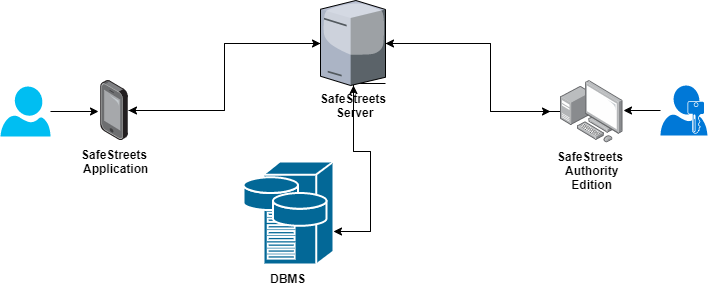
\includegraphics [scale=0.5] {diagrams/high-interaction.png}
			\caption[High-Level Interaction]{High-Level Interaction diagram}
			\label{fig:hinteraction_diagram}
		\end{figure}
		The figure describes how individuals interact with SafeStreets. Only one user is represented on the left and only one authority on the right, but this is only made to define clearly interactions. The real system is actually composed by multiple individuals.\\
		Basically everyone can download the SafeStreets application on his smartphone and can be an \textit{user}. On the other hand the Authority Edition is distributed by SafeStreets only to certificated \textit{authorities} that wants to collaborate with it. 
		\begin{figure}[H]
			\includegraphics [scale=0.5] {diagrams/High-level.png}
			\caption[High-Level Layers]{High-Level layers}
			\label{fig:hlayers}
		\end{figure}
		In figure \ref{fig:hlayers}	are defined three software logic layers on which the system is defined. \\
		The \textit{Individuals Layer} includes the two different kind of applications used by individuals. The distinction between applications is made because the two different implementation include different functionalities and, eventually, a different kind of interaction with the server with respect to the granularity of informations exchanged between them. \\
		The \textit{Server Layer} contains all the managerial components to interact correctly with individuals. It is also important as a security step. Indeed, individuals never communicate with the DBMS, that contains sensitive informations. They have to make requests to server and it manage them forwarding data requests to the DBMS. \\
		The \textit{Data Layer} is simply defined only by the data management system, that collects and execute queries from relational databases.
		\clearpage
		\subsection{Component view}
		Figure \ref{fig:component_diagram} represents all the components of SafeStreets ecosystem: SafeStreets App, SafeStreets AE (Authority Edition), SafeStreets Server and the database.\\
		The clients, so SafeStrees app and SafeStreetsAE, are not thin: they include part of the application logic. For example, the server receives violation reports the has already been validated by the app.
		\begin{figure}[H]
			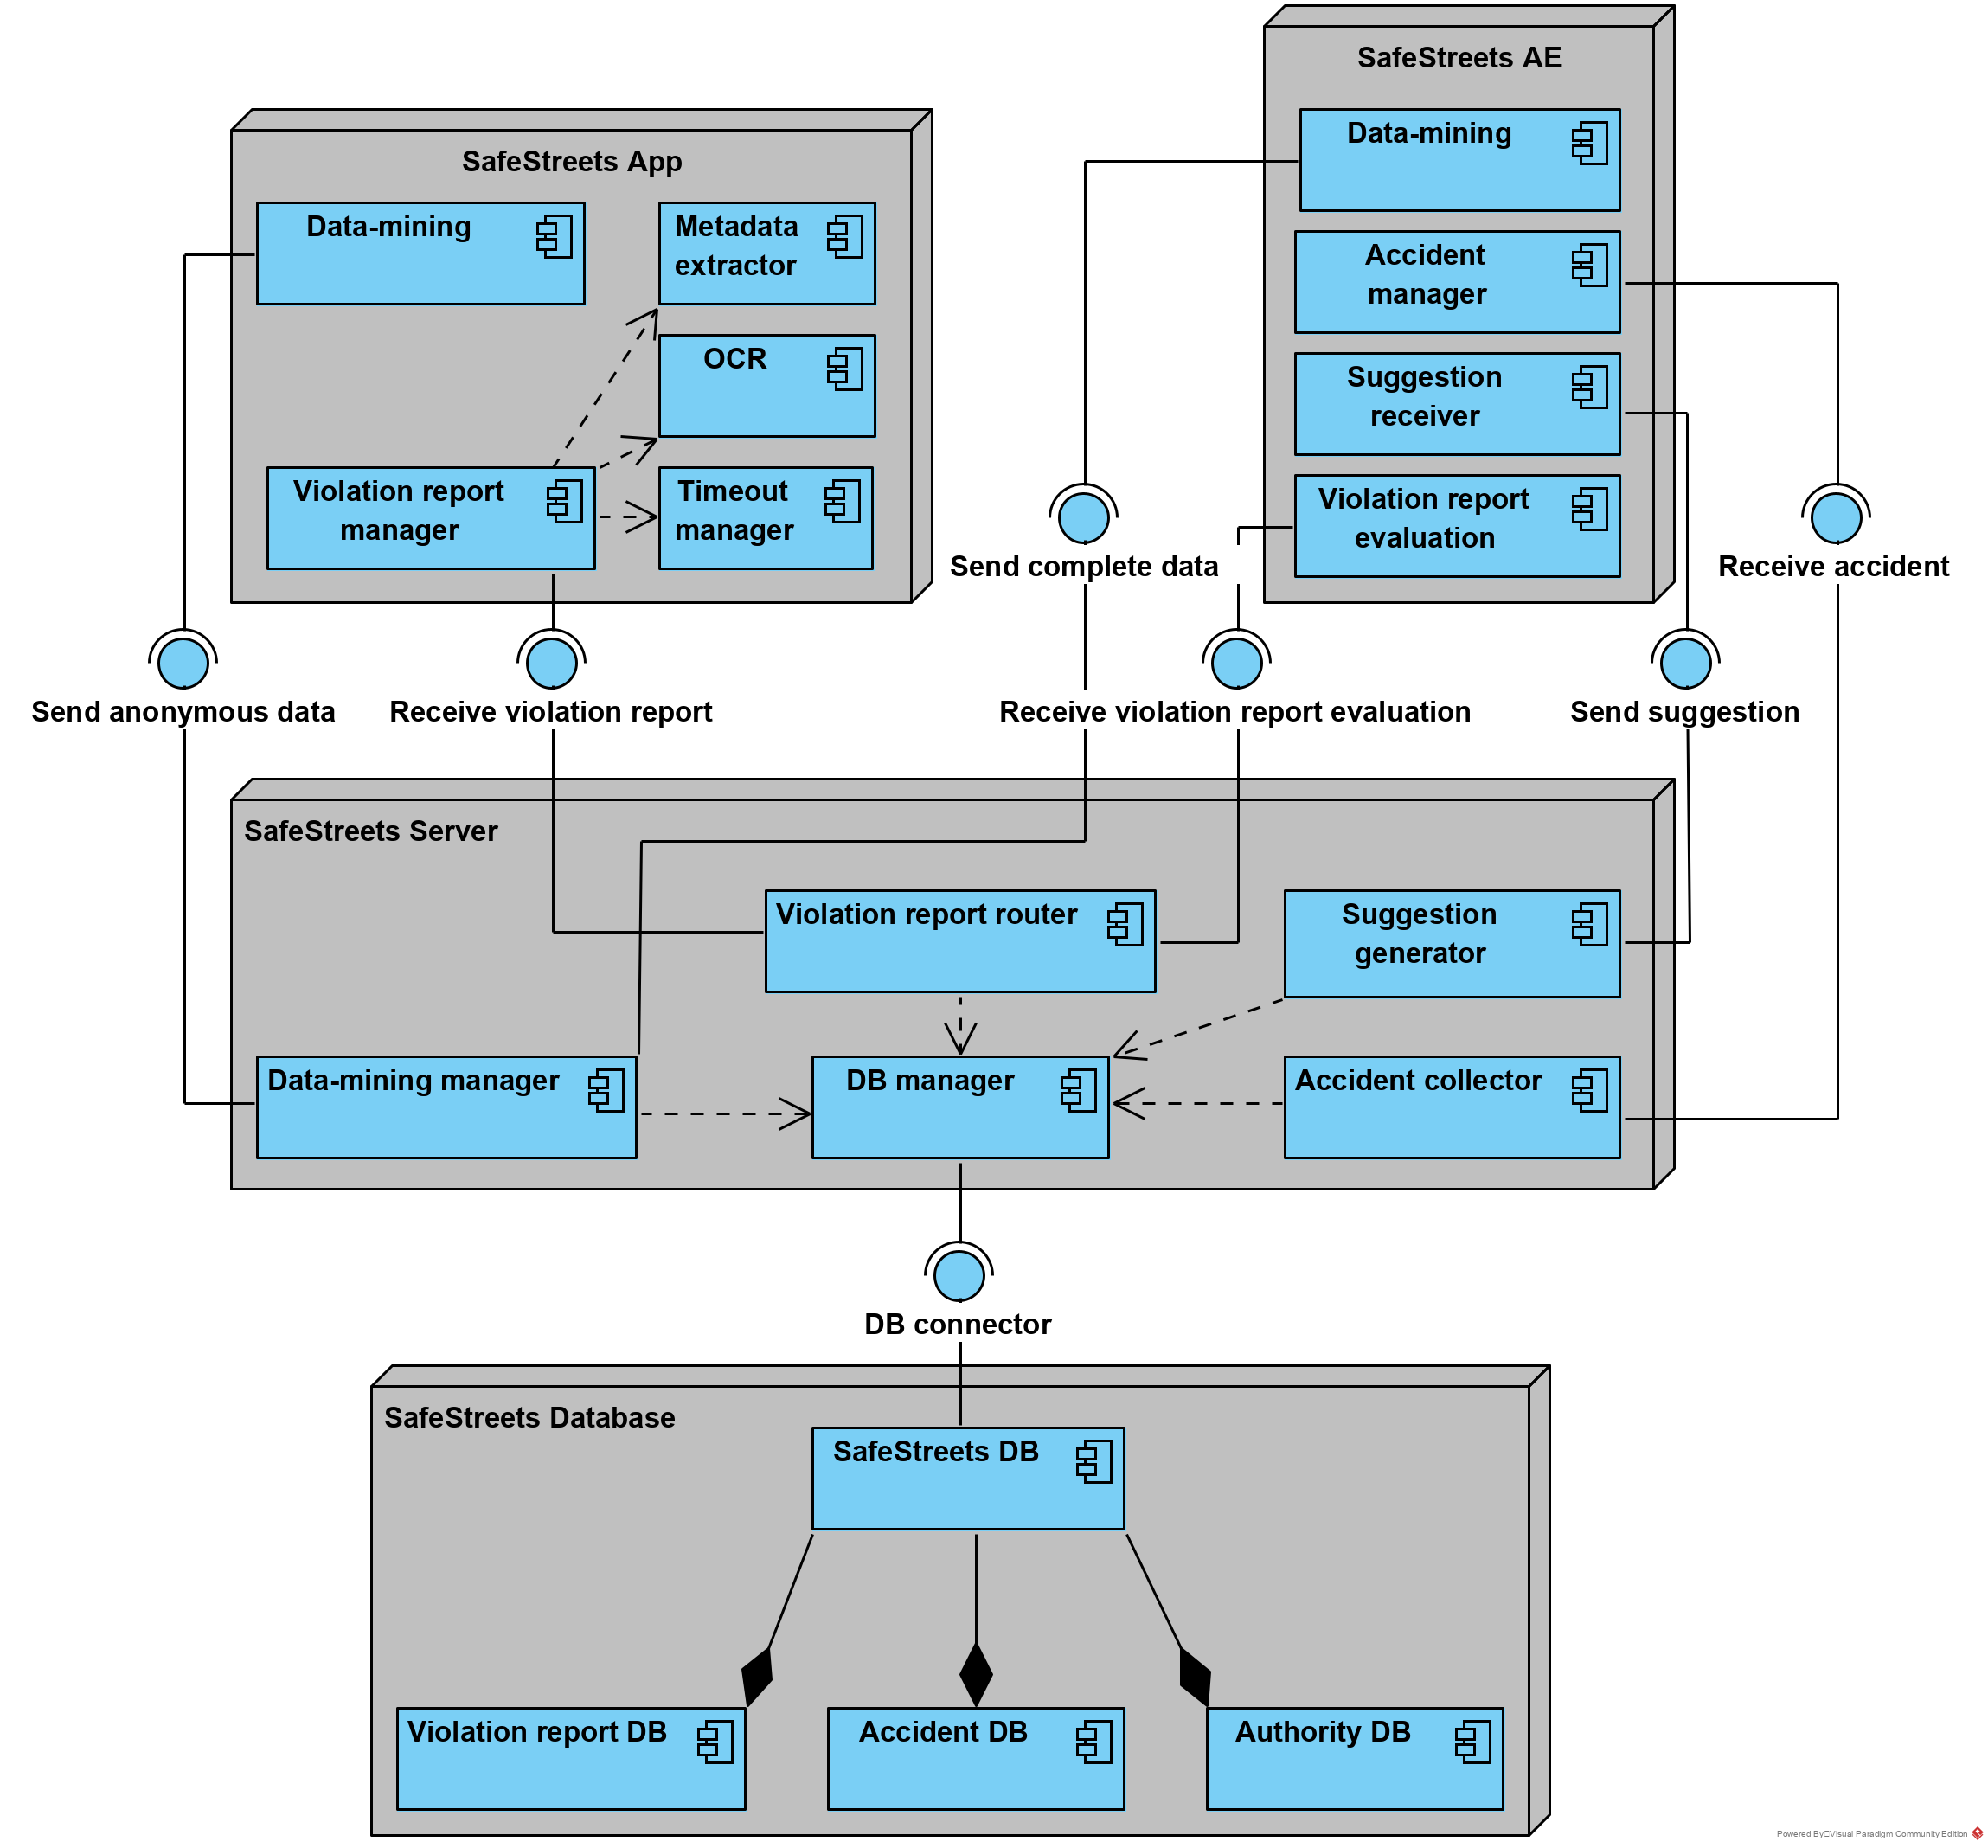
\includegraphics [scale=0.65] {diagrams/component_diagram.png}
			\caption[Component diagram]{Component diagram}
			\label{fig:component_diagram}
		\end{figure}
		
		\subsection{Deployment	view}
		\subsection{Runtime	view}
		\subsection{Component interfaces}
		\subsection{Selected architectural styles and patterns}
		\subsection{Other design decision}
	\clearpage	
	\section{User Interface Design}
	To give an approximate idea of how the interfaces of the application should appear, some mockups, both for SafeStreets Application and SafeStreets AE, have been given in \href{run:d:../DeliveryFolder/RASD1.pdf}{RASD} [Section 3.1.1].\\ 
	In order to express the relations among pictures RASD [3.1.1], here it will be illustrated a pair of UX Diagrams.
	
	\begin{figure}[H]
		\centering
		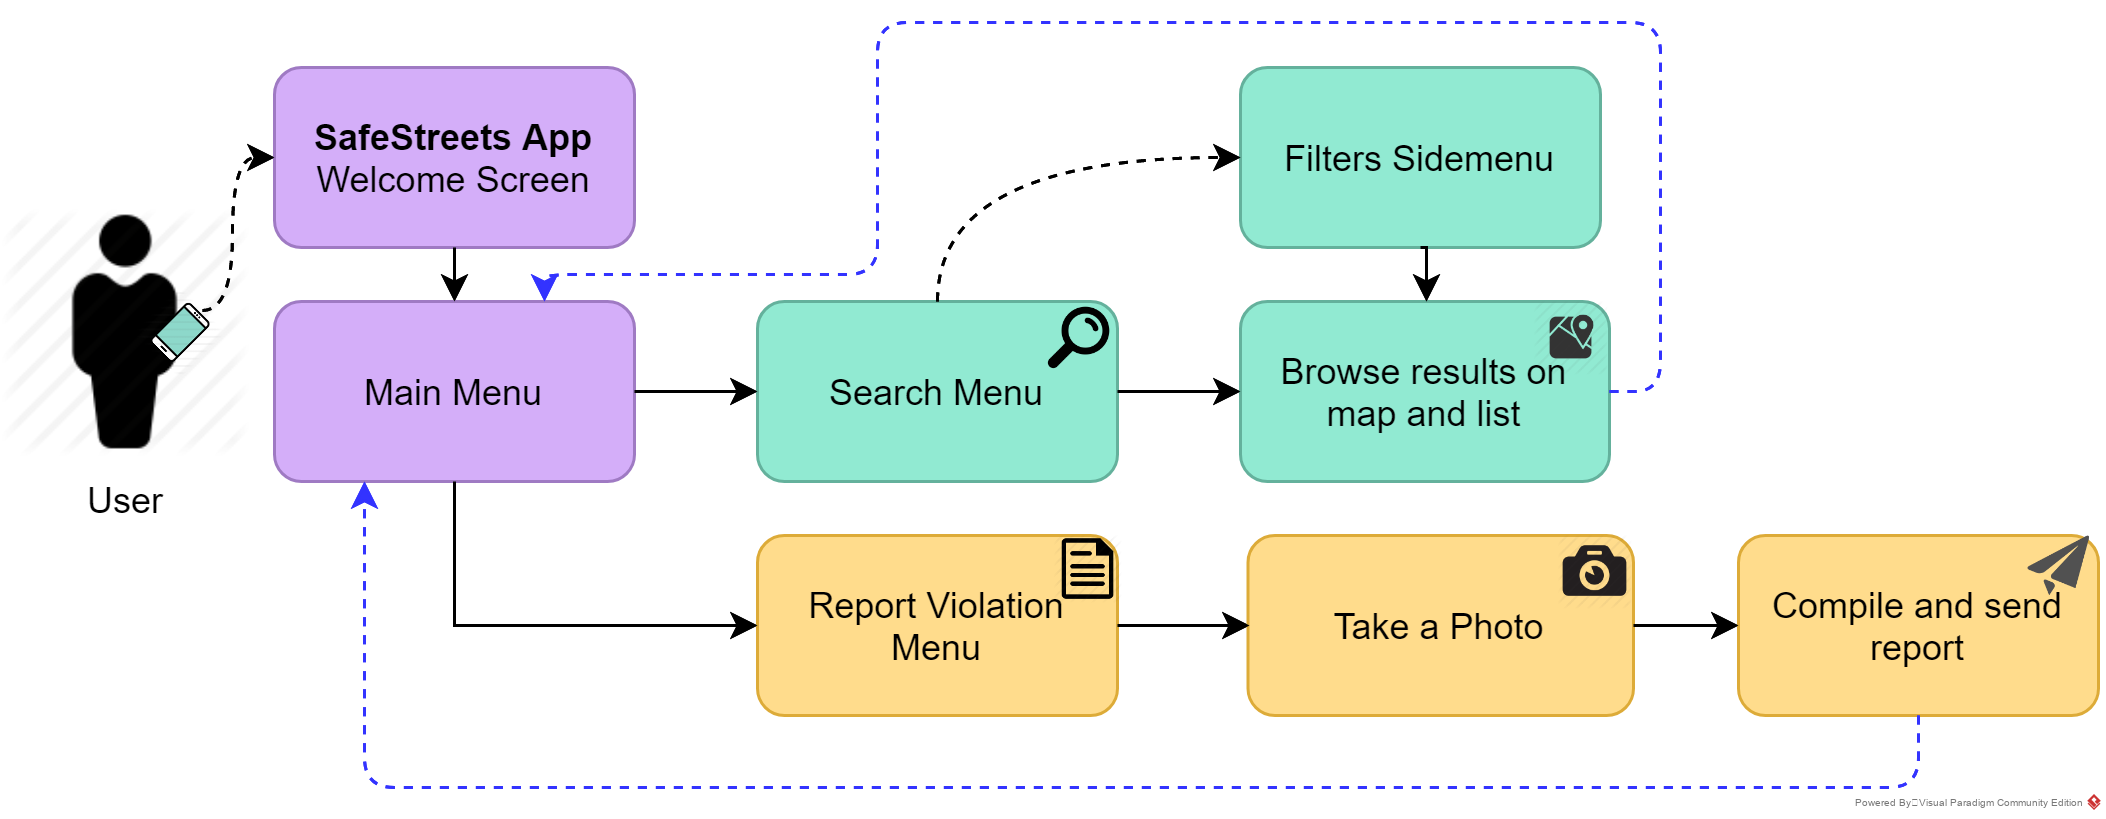
\includegraphics[width=1\textwidth]{diagrams/UXSafeStreetsApp.png}
		\caption[User Experience diagram for SafeStreets App]{User Experience diagram for SafeStreets App}
		\label{fig:UX_SSApp}
	\end{figure}

	\begin{figure}[H]
		\centering
		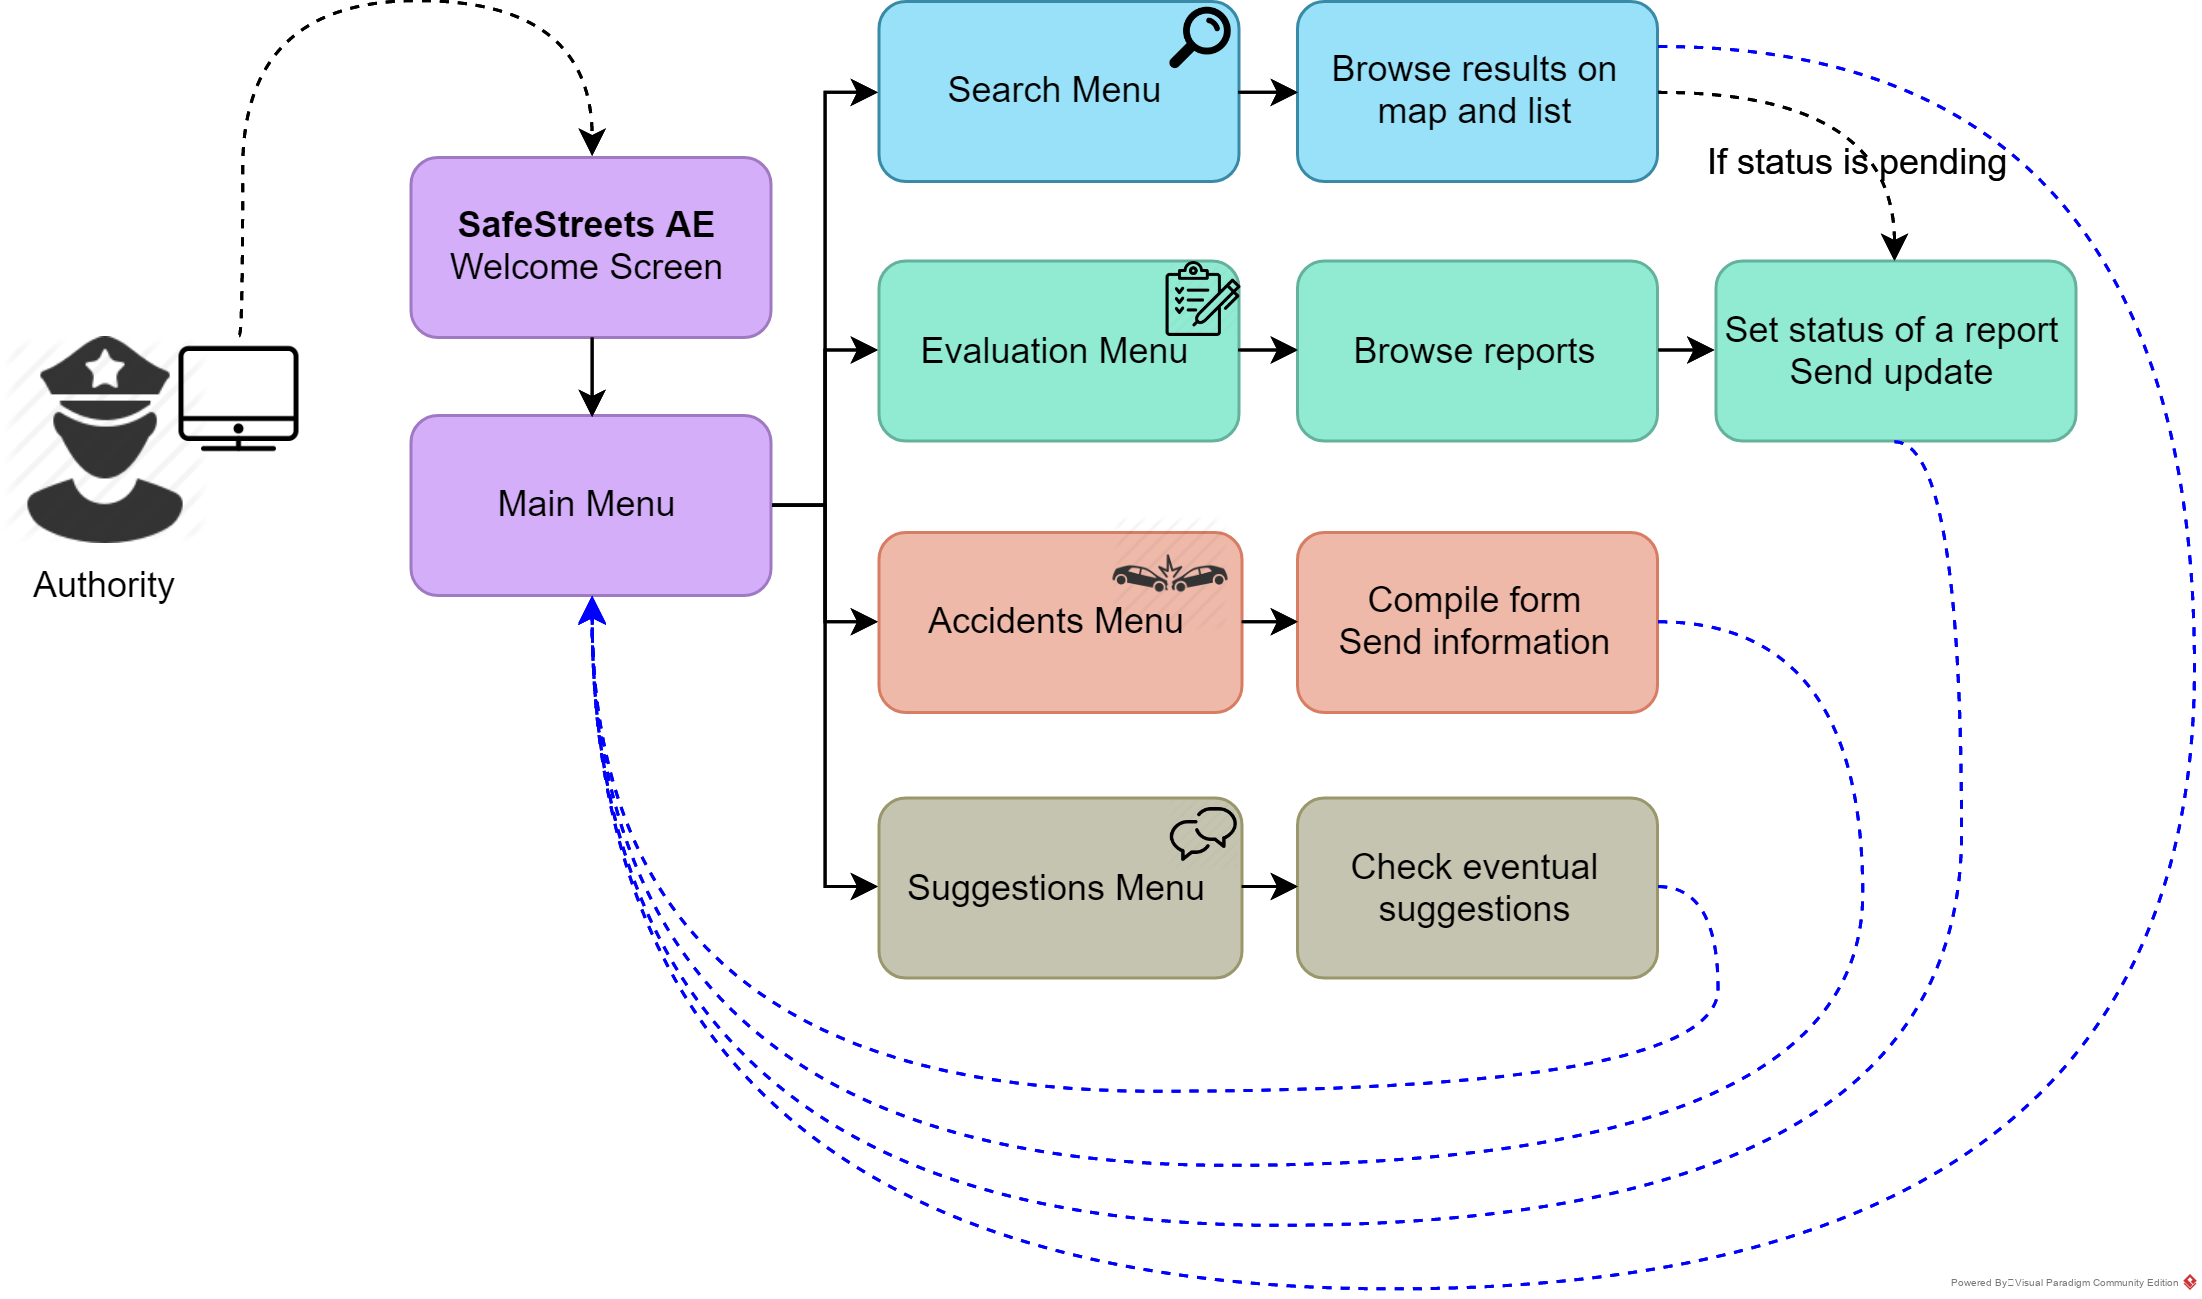
\includegraphics[width=1\textwidth]{diagrams/UXSafeStreetsAE.png}
		\caption[User Experience diagram for SafeStreets AE]{User Experience diagram for SafeStreets AE}
		\label{fig:UX_SSAE}
	\end{figure}
		
	\clearpage	
	\section{Requirements Traceability}
	\clearpage	
	\section{Implementation, integration and test plan}
	
	\clearpage
	\section{Effort Spent}
		\begin{table}[h]
			\centering
			\begin{tabular}{l c}
				\hline\hline
				\multicolumn{2}{c}{\textbf{Team Work}} \\
				\hline
				\textbf{Task} & \textbf{Hours} \\ [0.5ex]
				\hline
				Understanding the problem & 2  \\
				Brainstorming & 4 \\
				Software system attributes & 8 \\
				\hline
				\textbf{Total} & 14  \\
				\hline
			\end{tabular}
			\caption{Time spent by all team members}
			\label{fig:Time spent by all team members}
		\end{table}
		
		\begin{table}[h]
			\centering
			\begin{tabular}{l c l c l c}
				\hline\hline
				\multicolumn{6}{c}{\textbf{Individual Work}} \\
				\hline
				\multicolumn{2}{c |}{\textbf{Nicolò Sala}}  &
				\multicolumn{2}{c |}{\textbf{Sebastiano Quacquarelli}} &
				\multicolumn{2}{c}{\textbf{Simone Ricchiuti}}\\
				\hline
				\textbf{Task} & \textbf{Hours}
				& \textbf{Task} & \textbf{Hours}
				& \textbf{Task} & \textbf{Hours} \\ [0.5ex]
				\hline
				%Nicolò								Sebastiano							Simone
				Constraints & 2						& Definitions & 1					& Introduction & 4
				\\\hline
				Definitions & 1						& User interfaces. & 5				& Product functions  & 4
				\\\hline
				UC description & 3					& Domain model & 4				    & User characteristics  & 0.5 
				\\\hline
				Performance req. & 1				& UC descr./diagrams & 4			& Functional req & 2 
				\\\hline
				Design constraints & 1				& Assumptions & 2					& UC description & 3  
				\\\hline
				Alloy & 9							& Sequence diagrams & 2				& Activity Diagrams  & 2  
				\\\hline
				\textbf{Total} & 17					& \textbf{Total} & 18				& \textbf{Total} & 15.5
				\\\hline
			\end{tabular}
			\caption{Time spent by each team member}
			\label{fig:Time spent by each team member}
		\end{table}
	
	\clearpage
	\section{References}
		\begin{itemize}
			\item "2019-2020 Software Engineering 2 mandatory project: goal, schedules and rules";
			\item TeXstudio (\url{https://www.texstudio.org}) to edit the LaTeX document;
			\item Visual Paradigm CE (\url{https://www.visual-paradigm.com/}) to create UML and ArchiMate diagrams.
		\end{itemize} 
	
\end{document}
